\section{Parallel Concepts}
\label{sec:par_con}
The concept of parallel computing is simple, despite the complex impression many get at first glance.
Parallel computing equates to many real life situations, in which a lot of work needs to be done by a lot of 
resources, in the quickest time possible. The bottom line in both is to keep as many of those resources busy
at one time as possible.

\subsection{Parallel Bingo}
\label{sec:bingo}
Let's consider a real world example. A group of a hundred mathematicians meet one night to play a game of 
bingo. Curious as mathematicians are, they realize that there are a finite amount of bingo boards. The group
then asks; for each sequence of numbers called, which boards are the best? Out of a certain amount of 
number sequences, which boards win the most?

The mathematicians start their experiement. A sequence of numbers is pre-recorded, and then one 
mathematician begins checking each board to see how many each each needs to get a win. But the other 
nintety-nine mathematicians begin to realize that only one doing all the work will take a while, and they might
as well help.

Each mathematician gets in line. At the front of the line, a unique bingo board is handed out, along with a 
paper with the number sequence for the current game. For each game, all the papers have the same number 
sequence. Each mathematician goes back to their table and begins marking the bingo board. When a bingo is
reached, the mathematician writes how many numbers in the sequence the board needed for the win. Lower is
better, of course. They then go to the back of the line, and will report their results when their turn comes again.

\begin{figure}[h]
	\begin{center}
		\includegraphics[width=50mm]{images/bingo.png}
		\caption{Mathematicians getting bingo boards, and returning to the end of the line with results} 
		\label{bingo}
	\end{center}
\end{figure}

\subsection{Speedup Introduction}
The biggest question in parallel computing or processes is, of course, how much faster is it? Formally, what is the \gls{speedup}? 
In Section \ref{sec:bingo}, for example, we would expect one hundred mathematicians to do the work of one 
mathematician in $1/100$th of the time. But reviewing Section \ref{sec:bingo}, is this actually the case? No,
in fact. Each of the one hundred mathematicians spent considerable time in line. Since one mathematician
doing all the work would have never spent time in line, the line time counts against any speedup the group
has otherwise. This leads to our first formal point with Amdahl's Law:

\begin{figure}[h]
	\begin{center}
		\LARGE
		\begin{tabular}{l r}
			$ A $		&	$ = \frac{1}{(1 - P) + \frac{P}{N}} $ \\
		\end{tabular}

		\normalsize
		\begin{tabular}{l l}
			$ where $  & \\
					&	$ P $ is the portion of the program that can be 'parallelized' \\
					&	$ N $ processors or workers \\
					&	$ (1 - P) $ is the sequential / serial portion (cannot be parallelized) \\
		\end{tabular}
		\caption{Amdah's Law. \cite{amdahl}} 
		\label{amdahl}
	\end{center}
\end{figure}
\normalsize

$ P $ informally is the portion of the program that can be split up into sections, each of which can be worked 
on simultaniously. The name for this process is \gls{paralellization}. Informally, Ahmdahl's Law shows that 
the higher $ P $, or portion of work that can be split up, the more beneficial adding more workers ($ N $) is. Too many workers, and the benefit decreases.

In the Section \ref{sec:bingo}, this makes sense. There is not much benefit committing too many more
mathematicians than bingo boards. The time spent processing bingo boards still improves, but the gain
shrinks compared to the constant time of totaling all the boards together. Amdahl's Law highlights the 
relationship between parallel work and workers, and we can see this relationship more formally graphed:

\begin{figure}[h]
	\begin{center}
		\includegraphics[width=80mm]{images/amdahl_graph01}
		\includegraphics[width=80mm]{images/amdahl_graph02}
		\caption{Speedup comparisons,} 
		\label{amdahl_graph}
	\end{center}
\end{figure}

Figure \ref{amdahl_graph} compares speedups of the theoretical bingo game. The graphs highlight two points
from Amdahl's Law; larger gains with larger $ P $ values, and the law of diminishing returns. The right graph
shows the benefits of parallelization when the time to process a bingo board is double what the left graph is.
As N approaches infinity, $ \frac{P}{N} $ approaches 0, so $ A $ approaches $\frac{1}{(1 - P)} $. 

In the bingo example, there may not be much to gain from this knowledge. But in more complicated problems,
this highlights one of the key goals of parallelization: decreasing $ (1 - P) $ and increasing $ P $. Informally,
taking as many of the processes out of the serial / sequential portion of the process, and getting them into
the parallel portion of the program. There are right and wrong ways of doing this, which this report will cover.
Processes or algorithms that already have high $ P $ values are 'embarrasingly parallel'.

\subsubsection{Maximizing P}
In Section \ref{sec:bingo}, serial time ( $ (1 - P) $ ) and parallelizable time ( $ P $ ) were accounted for. But 
overhead time was ignored. In the bingo example, this equals the time spent waiting in line. As more 
mathematicians ( $ N $ ) are added, overhead increases. Since waiting in line is not parallelizable, this adds 
to the serial time ( $ (1 - P) $ ). This is as true in theory as it is in real computing systems. The resulting 
equation is:

\begin{figure}[h]
	\begin{center}
		\LARGE
		\begin{tabular}{l r}
			$ A $		&	$ = \frac{1}{((1 - P) + (T_P * N)) + \frac{P}{N}} $ \\
		\end{tabular}

		\normalsize
		\begin{tabular}{l l}
			$ where $  & \\
					&	$ P $ is the portion of the program that can be 'parallelized' \\
					&	$ N $ processors or workers \\
					&	$ (1 - P) $ is the sequential / serial portion (cannot be parallelized) \\
					&	$ (T_P * N) $ is the overhead \\
		\end{tabular}
		\caption{Amdah's Law (Figure \ref{amdahl}) with Overhead. } 
		\label{amdahl_overhead}
	\end{center}
\end{figure}
\normalsize

This adds complexity to Amdahl's Law, but adds logical results to calculating speedups:

\begin{figure}[h]
	\begin{center}
		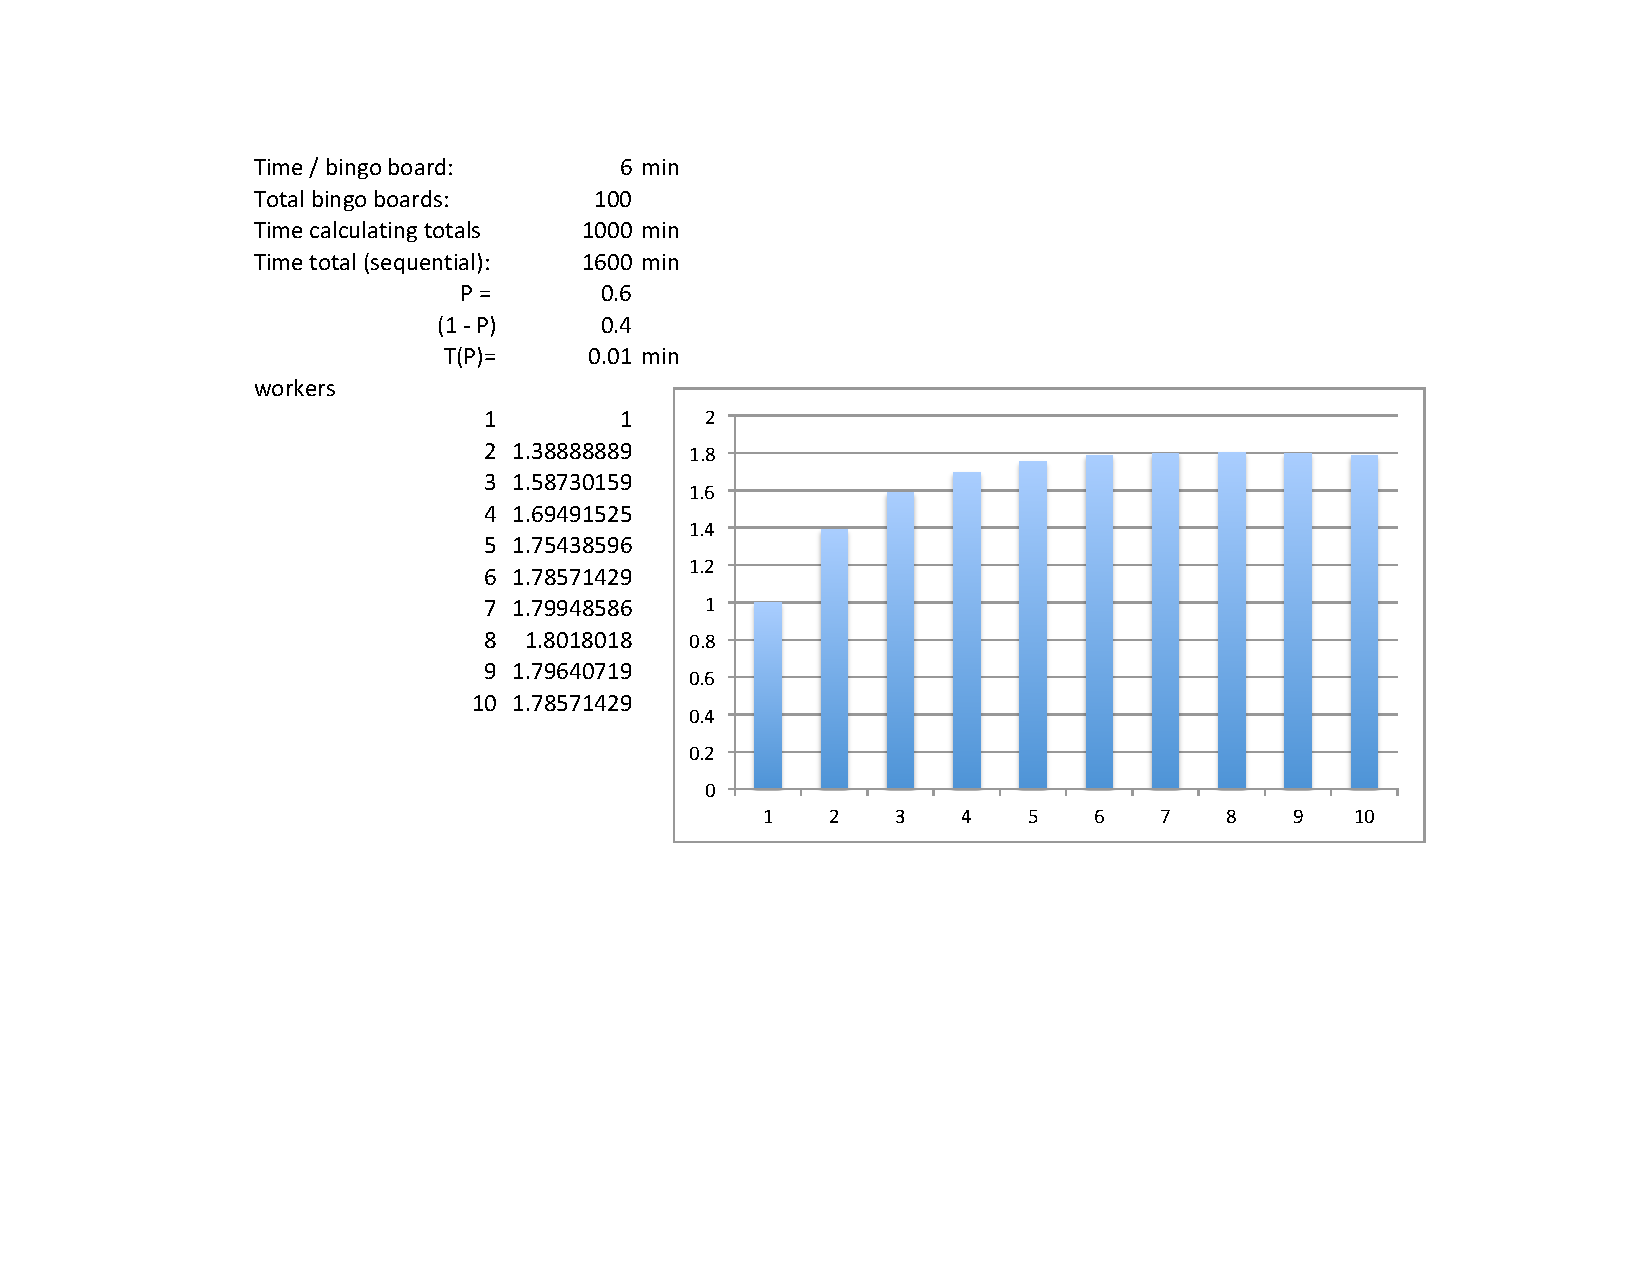
\includegraphics[width=130mm]{images/amdahl_overhead}
		\caption{Speedup comparisons including overhead} 
		\label{amdahl_overhead_graph}
	\end{center}
\end{figure}

Figure \ref{amdahl_overhead_graph} shows that not only the law of diminishing returns, but a negative 
benefit. Adding more workers actual slows parallel processes down at a certain point. In the bingo example,
at a certain point, adding more workers just creates longer lines and doesn't actually speed bingo board 
checking up. For many algorithms, $ P $ can only be a fairly small size. The best value for $ N $ will then only be 1. If $ P $ is not very big to begin with, than any $ N $ greater than 1 will cause a slowdown instead 
of speedup. Thus, even though some programs can be parallelized, if $ N > 1 $ causes a slowdown, they 
shouldn't.


\subsection{Speedup Summary}
Figure \ref{amdahl_overhead_graph} highlights two other key goals of parallelization: minimize $ T_P $, and 
maximize \gls{granularity} \cite{mit}. Granularity is how much work time each iteration or sub-process takes. 
In maximizing \gls{granularity}, $ P $ is maximized. In the bingo example, this means taking any process the 
totaller has to do at the end, and seeing if each mathematician can do it for their respective bingo board. This
saves the totaller time at the end, decreases serial time ( $ (1 - P) $ ), and increases parallel time ( $ P $ ).

The correct way to maximize $ P $ is to replace serial time processes with parallel time processes. The 
incorrect was is to simply inflate $ P $. If a process is not being moved from serial to parallel time, a bigger
$ P $ value will not lead to a real speedup. Informally, making more busy work for all the workers that doesn't
help reach the overall goal doesn't justify adding more workers. This may seem obvious, but is often 
attempted when $ N > 1 $ causes slowdowns. 

The analogy is that it is better to run optimized serial processes than it is to parallelize garbage. The former is
usually quicker anyway, and doesn't require more resources. This seems obvious, but the latter is often 
tried when parallelization is misinterpretted as a sledgehammer for making processes run faster.
